%TODO INTRODUCTION POUR LE TRUC
La méthode de Newton-Raphson est une méthode itérative permettant le calcul de racine d'une fonction en utilisant 
une approximation locale de la fonction $f$ par sa tangente en un point donné.
subsection{Définition}
La méthode de Newton-Raphson peut être définie de la manière suivante : \\
%% \begin{algorithm}
%% \caption{Méthode de Newton-Raphson}
%% \KwData{Une fonction $f : \mathbb{R}^n \to \mathbb{R}^m$ \\
%%         Un vecteur initial $U$ \\
%%         La matrice Jacobienne de $f$ notée $H$}
%% \KwResult{Un vecteur $U$ approximant une racine de $f$}
%% \While{non convergence de la solution}{
%%     Calculer $f(U)$ et $H(U)$\;
%%     Soit $V$
%%     Résoudre $H(U) V = -f(U)$ pour $V$\;
%%     Mettre à jour $U \gets U + V$\;
%%     $k \gets k + 1$\;
%% }
%% \Return{$U$}
%% \end{algorithm}
\begin{itemize}
  \item Soit la fonction continue  $f$ : $ \mathbb{R}^n \to \mathbb{R}^m $
  \item Soit $ H $ la jacobienne de $f$.
  \item Soit un vecteur arbitraire de $\mathbb{R}^n$.
\end{itemize}
On cherche le vecteur $V$ qui résout le système non linéaire : $f(U + V) = 0$.\\
Le vecteur $U$ est alors actualisé en utilisant $V$: $U \gets U + V$ \\
La méthode est répétée jusqu'à une convergence de la solution $U$, soit lorsque $||f(U)|| < \epsilon$.



\subsection{Méthode de calcul de $V$}
La définition actuelle de $V$ ne permet pas un calcul numérique de $V$ simple.
Nous allons donc définir une relation entre $H, U$ et $ V$ permettant ce calcul.
En utilisant l'approximation :
\[
f(U + V) \approx f(U) + H(U)\cdot V
\]
Or, par définition $V$ est le vecteur tel que $f(U + V ) = 0$, donc on en déduit : $f(U) + H(U)\cdot V \approx 0 $
Calculer $V$ revient à résoudre le système linéaire :
\[
H(U)\cdot V = -f(U)
\]
Cette résolution peut se calculer numériquement grâce à des librairies Python telles que Numpy \citep{numpy_equalin}.
%Sachant que $f(U + V ) = 0$ et $f(U + V)$ est approximée par $f(U) + H(U)\cdot V$ \\
%On trouve alors que \[
%H(U)\cdot V \approx - f(U)
%\]
%Parler du backtracking


\subsection{Backtracking}
En réécrivant l'équation $H(U)\cdot V = -f(U)$, nous obtenons : 
\[ V = -H(U)^{-1}\cdot f(U) \]
L'inverse de la jacobienne de $f$ n'étant pas définie continue, les valeurs singulières de cette dernière peuvent entraîner des étapes instables et conduire à une divergence de la méthode.\\
Nous pouvons utiliser le principe de "backtracking" afin de garantir une convergence de la solution.\\
En utilisant la condition d'Armijo : $ || f(U+t\cdot V)|| > || f(U) + \alpha \cdot t \cdot ||V||$
\\
\begin{itemize}
  \item $t \in [0,1]$ le pas de réduction 
  \item $\alpha \in [0,1] $ le degré d'erreur induite acceptable
\end{itemize}
Nous pouvons itérer en actualisant la valeur de $t$  d'un facteur $\beta \in [0,1[$ jusqu'à ce que la condition soit fausse.\\ 
La valeur de la prochaine itération de $U$ dans la méthode de Newton-Raphson est alors proportionnelle à $t$  : $U = U + t\cdot V$.

\subsection{Vitesse de convergence}

La méthode de Newton-Raphson est réputée pour sa convergence quadratique, ce qui signifie que l'erreur entre l'approximation actuelle et la solution exacte diminue approximativement au carré à chaque itération, sous hypothèse de régularité de $f$.  

Plus précisément, si $U_k$ est l'approximation à l'itération $k$ et $U^*$ la solution exacte, alors dans les cas favorables, l'erreur $\| U_{k+1} - U^* \|$ satisfait la relation suivante :  
\[
\| U_{k+1} - U^* \| \leq C \| U_k - U^* \|^2
\]
où $C$ est une constante dépendant de la fonction $f$. Cette propriété implique une amélioration exponentielle de la précision au fil des itérations.  

Le graphique \ref{fig:convergence_newton} illustre cette convergence rapide en montrant la décroissance de la norme de l'erreur $\| f(U_k) \|$ au fil des itérations :

\begin{figure}[h]
    \centering
    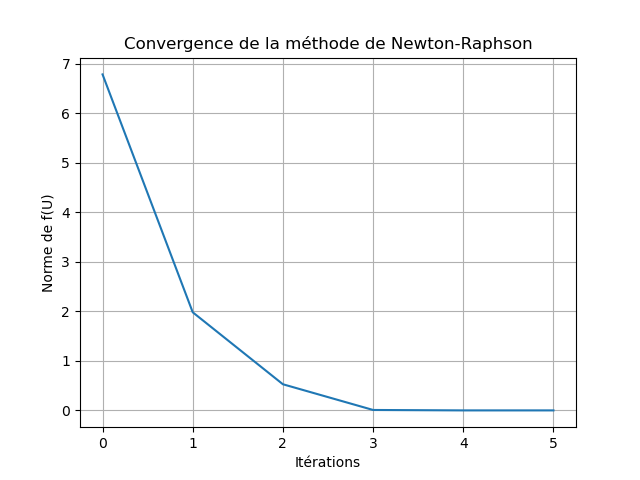
\includegraphics[width=0.8\textwidth]{newton_raphson_convergence.png}
    \caption{Illustration de la convergence quadratique de la méthode de Newton-Raphson}
    \label{fig:convergence_newton}
\end{figure}

\newpage
On constate que, après quelques itérations, l'erreur diminue de manière significative, ce qui confirme la nature quadratique de la convergence et l'efficacité de la méthode dans les cas où elle est applicable.
